\documentclass{beamer}
\usetheme{CambridgeUS}

\begin{document}

%Stage 0: About me

%PART1

%Stage 1: Introduction
%Stage 2: The good parts
%Bonus stage 1: Installing Node.js
%Stage 3: Manage your dependencies with Bower
%Stage 4: Automate your workflow with Grunt
%Stage 5: Basic HTML5 game development: the game loop

%PART2

%Stage 6: Refactor our client-side code with Require.js
%Stage 7: Events, events everywhere
%Stage 8: Multiplayer game with Node.js and socket.io
%Stage 9: Finish gameplay and deploy
%Stage 10: Persistance with RedisDB

\title{Javascript, The Swiss Army Knife of Programming Languages}
\author{David Morcillo}
\date{23-11-2013}

\begin{frame}
  \titlepage
\end{frame}

\section{Stage 0: About me}

\begin{frame}
  \frametitle{About me}
  
\includegraphics[width=150px]{images/bastard_david.jpg}
  \begin{itemize}
    \item twitter.com/ultrayoshi
    \item github.com/ultrayoshi
  \end{itemize}
\end{frame}

\section{Stage 1: Introduction}

\begin{frame}
\end{frame}

\begin{frame}
  \frametitle{Features}

  \begin{itemize}
    \item Loosely typed language
    \pause\item Object literal notation
    \pause\item Prototypal inheritance
    \pause\item Global variables
    \pause\item Functions are first class objects
  \end{itemize}
\end{frame}

\begin{frame}
  \frametitle{Features}

  \begin{block}{ECMAScript}
    The standard that defines JavaScript is the third edition of \textit{ECMAScript Programming Language}.
  \end{block}
\end{frame}

\begin{frame}[fragile]
  \frametitle{Hello World}

  \begin{block}{index.html}
    {\scriptsize
    \begin{verbatim}
    <html>
      <head>
        <script>
          document.writeln(``Hello, world!'');
        </script>
      </head>
      <body>
      </body>
    </html>
    \end{verbatim}
    }
  \end{block}
\end{frame}

\begin{frame}[fragile]
  \frametitle{Syntax}

  \begin{block}{Comments}
  Block comments formed with /* */ and line-ending comments starting with //. Example:
  {\scriptsize
  \begin{verbatim}
  /* 
    We are learning Javascript and comments are very important
  */
  document.writeln(``Hello World!''); // Output: Hello World!
  \end{verbatim}
  }
  \end{block}

  \pause
  
  \begin{block}{Names}
    Starts with a letter or underscore and optionally followed by on or more letters, digits or underscores. Beware of some reserved words.
    {\scriptsize
    \begin{verbatim}
    bullet           // valid     _mana            // valid
    3force 	         // invalid   lucky42          // valid
    rocket-launcher  // invalid   grenade_launcher // valid
    \end{verbatim}
    }
  \end{block}
\end{frame}

\begin{frame}[fragile]
  \frametitle{Syntax}

  \begin{block}{Numbers}
    Single number type represented internally as 64-bit floating point.
    {\scriptsize
    \begin{verbatim}
    42 
    3.141516
    10e5
    1/0 // Output: Infinity
    0/0 // Output: NaN
    \end{verbatim}
    }
  \end{block}

  \pause

  \begin{block}{Strings}
    Can be wrapped in single quotes or double quotes. It can contains 0 or more characters. All characters in Javascript are 16 bits wide.
    {\scriptsize
    \begin{verbatim}
    ``Hello World''
    'Hello World'
    ``This is\n a multiline string''
    'You can write `` on single quotes string'
    \end{verbatim}
    }
  \end{block}
\end{frame}

\begin{frame}[fragile]
  \frametitle{Syntax}

  \begin{block}{Functions}
  {\scriptsize
  \begin{verbatim}
  function helloWorld (name) {
      console.log('Hello ' + name + '!');
  }

  helloWorld('David'); // Output 'Hello David!'

  var myFunction = function () {
      console.log('Hi there!');
  };

  myFunction(); // Output: 'Hi there!'
  \end{verbatim}
  }
  \end{block}
\end{frame}

\begin{frame}[fragile]
  \frametitle{Syntax}

  \begin{block}{Variables}
    Use the \texttt{var} keyword followed by a name to declare a variable. When used inside of a function, the \texttt{var} statement defines the function's private variables.
    {\scriptsize
    \begin{verbatim}
    var player; // variable player declared on a global scope

    function test() {
        var enemy; // Scoped to function test

        function test2() {
            var bullet;  // Scoped to function test2
        }
    }
    \end{verbatim}
    }
  \end{block}
\end{frame}

\begin{frame}[fragile]
  \frametitle{Syntax}

  \begin{block}{\texttt{if}, \texttt{else}}
    \scriptsize{
    \begin{verbatim}
    var testOk = true;

    if (testOk) {
        console.log(``Captain obvious'');
    } else {
        console.log(``I'm bored'');
    }
    \end{verbatim}
    }
    Here are the \textit{falsy} values:
    \begin{itemize}
      \item \texttt{false}
      \item \texttt{null}
      \item \texttt{undefined}
      \item The empty string
      \item The number 0
      \item The number NaN
    \end{itemize}
    All other values are \textit{truthy}.
  \end{block}
\end{frame}

\begin{frame}[fragile]
  \frametitle{Syntax}

  \begin{block}{\texttt{switch}}
    \scriptsize{
    \begin{verbatim}
    var weapon = ``rocketlauncher'';

    switch(weapon) {
        case ``pistol'':
            console.log(``piu piu'');
            break;
        case ``shotgun'':
            console.log(``paaam!'');
            break;
        case ``rocketlauncher''
            console.log(``BOOOOM!'');
            break;
        default:
            console.log(``falcon punch!'');
            break;
    }
    \end{verbatim}
    }
  \end{block}
\end{frame}

\begin{frame}[fragile]
  \frametitle{Syntax}

  \begin{block}{\texttt{while}, \texttt{do while}}
    \scriptsize{
    \begin{verbatim}
    var counter = 0;
    while (counter < 10) { // Ends when counter is equal to 10
        console.log(counter);
        counter += 1;
    }

    do {
        console.log(counter);
        i -= 1;
    } while(counter > 0); // Ends when counter is equal to 0
    \end{verbatim}
    }
  \end{block}

  \pause

  \begin{block}{\texttt{for}}
    {\scriptsize
    \begin{verbatim}
    var i;

    for (i = 0; i < 10; i += 1)
        console.log(i);
    }
    \end{verbatim}
    }
  \end{block}
\end{frame}

\section{Stage 2: The good parts}

\begin{frame}[fragile]
  \begin{center}
    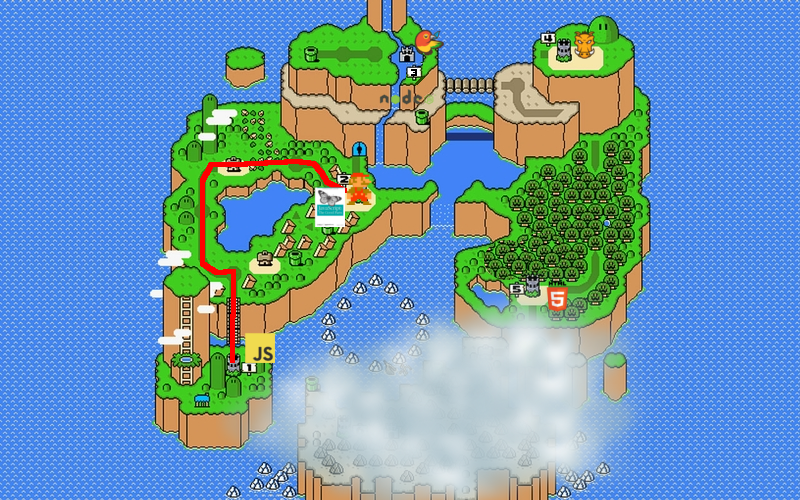
\includegraphics[width=300px]{images/map_stage_2.png}
  \end{center}
\end{frame}

\begin{frame}[fragile]
  \frametitle{Objects}
  \begin{itemize}
    \item Objects in Javascript are mutable keyed collections.
    \pause\item Arrays, functions and regular expressions are objects.
    \pause\item A property name can be any string.
    \pause\item Objects can inherit properties of another through its prototype.
  \end{itemize}

  \pause

  \begin{block}{\texttt{Prototype}}
    All objects created from object literals are linked to \texttt{Object.prototype}.
    \pause

    If we try to retrieve a property value from an object, and if the object lacks the property name, then Javascript attempts to retrieve the property value from the prototype object.
  \end{block}
\end{frame}

\begin{frame}[fragile]
  \frametitle{Objects}
  \begin{block}{\texttt{Object.create}}
    {\scriptsize
    \begin{verbatim}
    var soldier = {
        hp: 10,
        strength: 5,
        weapon: 'Pistol'
    };

    var knight = Object.create(soldier);
    knight.weapon = 'Sword';
    knight.shield = true;

    console.log(knight.hp); // Output: 10
    console.log(knight['weapon']); // Output: 'Sword'
    console.log(knight.shield); // Output: true
    \end{verbatim}
    }
  \end{block}

  Visit \url{http://www.objectplayground.com/} for a graphical explanation
\end{frame}

\begin{frame}[fragile]
  \frametitle{Objects}
  \begin{block}{\texttt{hasOwnProperty}}
    {\scriptsize
    \begin{verbatim}
    console.log(knight.hasOwnProperty('hp')); // Output: false
    console.log(knight.hasOwnProperty('shield')); // Output: true
    \end{verbatim}
    }
  \end{block}

  \pause

  \begin{block}{\texttt{for in}}
    {\scriptsize
    \begin{verbatim}
    for (attr in knight) {
        if(knight.hasOwnProperty(attr)) {
            console.log('Knight property ' + attr + ' with value ' + 
                knight[attr]);  
        }
    }
    // Knight property weapon with value 'Sword'
    // Knight property shield with value true
    \end{verbatim}
    }
  \end{block}
  
  \pause

  \begin{block}{\texttt{delete}}
    {\scriptsize
    \begin{verbatim}
    console.log(knight.weapon); // Output: 'Sword'
    delete knight.weapon;
    console.log(knight.weapon); // Output: 'Pistol'
    \end{verbatim}
    }
  \end{block}
\end{frame}

\begin{frame}[fragile]
  \frametitle{Functions}

  Functions are the \textbf{fundamental modular unit} of Javascript. They are used for code reuse, information hiding, and composition. \\

  The thing that is special about functions is that they can be invoked.
  \pause

  \begin{block}{Function.prototype and constructor}
  Functions are objects linked to Function.prototype. Every function object is also created with a prototype property. Its value is an object with a constructor property whose value is the function.
  \end{block}

  \pause
\end{frame}

\begin{frame}[fragile]
  \frametitle{Functions}

  Invoking a function suspends the execution of the current function, passing control and parameters to the new function. In addition to the declared parameters, every function receives two additional parameters: \texttt{this} and \texttt{arguments}.

  \pause

  \begin{block}{Invocation (1/4): Method invocation pattern}
    {\scriptsize
    \begin{verbatim}
    var enemy = {
        hp: 5,
        rage: 0,
        attack: function () {
            this.rage += 1;
        }
    };

    enemy.attack();
    console.log(enemy.rage); // Output: 1
    \end{verbatim}
    }
  \end{block}
\end{frame}

\begin{frame}[fragile]
  \frametitle{Functions}

  \begin{block}{Invocation (2/4): Function invocation pattern}
    {\tiny
    \begin{verbatim}
    // part of code omitted
    physicsManager.collisionsDetected = 0;
    physicsManager.checkCollision = function (entity1, entity2) {
        var bbCollision = function (bb1, bb2) {
            // Collision code omitted
            var collision = true;
            if (collision) {
                // WARNING: 'this' is the global object and not 'physicsManager'
                this.collisionsDetected += 1;
            }
            return collision;
        };

        bbCollision(entity1.getBB(), entity2.getBB());
    };

    if (physicsManager.checkCollision(enemy, player)) {
        player.takeDamage(enemy.strength);
    }

    console.log(physicsManager.collisionsDetected); // Output: 0
    \end{verbatim}
    }
  \end{block}
\end{frame}

\begin{frame}[fragile]
  \frametitle{Functions}

  \begin{block}{Invocation (2/4): Function invocation pattern (workaround)}
    {\scriptsize
    \begin{verbatim}
    physicsManager.collisionsDetected = 0;

    physicsManager.checkCollision = function (entity1, entity2) {
        var that = this;

        var bbCollision = function (bb1, bb2) {
            // Collision code omitted
            var collision = true;
            if (collision) {
                that.collisionsDetected += 1;
            }
            return collision;
        };

        bbCollision(entity1.getBB(), entity2.getBB());
    };

    if (physicsManager.checkCollision(enemy, player)) {
        player.takeDamage(enemy.strength);
    }

    console.log(physicsManager.collisionsDetected); // Output: 1
    \end{verbatim}
    }
  \end{block}
\end{frame}

\begin{frame}[fragile]
  \frametitle{Functions}

  \begin{block}{Invocation (3/4): Constructor invocation pattern}
    {\scriptsize
    \begin{verbatim}
    var Player = function (name) {
        this.name = name;
        this.lives = 3;
    };

    Player.prototype.sayMyName = function () {
        console.log('My name is ' + this.name);
    };

    var david = new Player('David');
    david.sayMyName(); // Output: 'My name is David'
    \end{verbatim}
    }
  \end{block}
\end{frame}

\begin{frame}[fragile]
  \frametitle{Functions}

  \begin{block}{Invocation (3/4): Constructor invocation pattern (without new)}
    {\scriptsize
    \begin{verbatim}
    var Player = function (name) {
        this.name = name;
        this.lives = 3;
    };

    Player.prototype.sayMyName = function () {
        console.log('My name is ' + this.name);
    };

    var manfred = Player('Manfred'); // oops
    try {
        manfred.sayMyName(); // raise an error because manfred is undefined
    } catch (e) {
        console.log('[' + e.name + '] ' + e.message);
    }
    
    // Global variables feast
    console.log(name); // Output: 'Manfred'
    console.log(lives); // Output: 3
    \end{verbatim}
    }
  \end{block}
\end{frame}

\begin{frame}[fragile]
  \frametitle{Functions}

  \begin{block}{Invocation (4/4): Apply invocation pattern}
    {\scriptsize
    \begin{verbatim}
    var enemy = {
        rage: 0,
        attack: function () {
            this.rage += 1;
        }
    };

    var anotherEnemy = {
        rage: 10
    };

    enemy.attack.apply(anotherEnemy, []);

    console.log(anotherEnemy.rage); // Output: 11
    \end{verbatim}
    }
  \end{block}
\end{frame}

\begin{frame}[fragile]
  \frametitle{Functions}

  \begin{block}{\texttt{Arguments}}
  {\scriptsize
  \begin{verbatim}
  function doActions() {
      var i, l;

      // WARNING: arguments is an Array-like object
      for (i = 0, l = arguments.length; i < l; i += 1) {
          console.log('Doing action ' + arguments[i]);
      }
  }

  doActions('jump', 'attack');
  /*
      Output:
      'Doing action jump'
      'Doing action attack'
  */
  \end{verbatim}
  }
  \end{block}
\end{frame}

\begin{frame}[fragile]
  \frametitle{Functions}

  \begin{block}{Closure}
  Javascript does have function scope. That means that the parameters and variables defined in a function are not visible outside of the function, and that a variable defined anywhere within a function is visible everywhere within the function.
  {\scriptsize
  \begin{verbatim}
  var player = new Player();

  function isGameOver() {
      var enemy = new Enemy();

      function checkHit() {
          return enemy.hit(player);
      }

      return checkHit();
  }

  isGameOver();
  \end{verbatim}
  }
  \end{block}

\end{frame}

\begin{frame}[fragile]
  \frametitle{Functions}
  \begin{block}{Module pattern}
  {\tiny
  \begin{verbatim}
  var physicsModule = (function () { // IIEF pattern
     var detectedCollisions = 0;

     function checkBBCollision(bb1, bb2) {
        var collision = false;
        // collision code skipped
        if (collision) {
            detectedCollisions += 1;
        }
        return collision;
     }

     function checkCollision(entity1, entity2) {
        checkBBCollision(entity1.getBB(), entity2.getBB());
     }

     return {
        checkCollision: checkCollision
     };
  }());

  console.log(physicsModule.detectedCollisions); // Output: undefined
  console.log(physicsModule.checkBBCollision); // Output: undefined
  console.log(typeof physicsModule.checkCollision); // Output: 'function'
  \end{verbatim}
  }
  \end{block}
\end{frame}

\begin{frame}[fragile]
  \frametitle{Inheritance}

  Javascript provides a much richer set of code reuse patterns. It can ape the classical pattern, but it also supports other patterns that are more expressive.

  \pause

  \begin{block}{Javascript is a class-free language}
    In classical languages, objects are instances of classes, and a class can inherit from another class. Javascript is a prototypal language, which means that objects inherit directly from other objects.
  \end{block}
  
\end{frame}

\begin{frame}[fragile]
  \frametitle{Inheritance}

  \begin{block}{Pseudoclassical pattern}
  {\tiny
  \begin{verbatim}
  var Alien = function (name) {
      this.name = name;
  };

  Alien.prototype.talk = function () {
      console.log('%?saf? ' + this.name);
  };

  var SmartAlien = function (name) {
      this.name = name;
  };

  SmartAlien.prototype = new Alien();

  SmartAlien.prototype.speech = function () {
      this.talk();
      console.log('...I mean, my name is ' + this.name);
  };

  var enemy = new SmartAlien('Roger');
  enemy.speech(); 
  // Output: '%?saf? Roger
  //         ...I mean, my name is Roger'
  \end{verbatim}
  }
  \end{block}
\end{frame}

\begin{frame}[fragile]
  \frametitle{Inheritance}

  \begin{block}{Prototypal pattern}
  {\tiny
  \begin{verbatim}
  var alien = {
      name: '%?&789',
      talk: function () {
          console.log('%?saf? ' + this.name);
      }
  };

  var smartAlien = Object.create(alien);
  smartAlien.speech = function () {
      this.talk();
      console.log('...I mean, my name is ' + this.name);
  };

  var enemy = Object.create(smartAlien);
  enemy.name = 'Roger';
  enemy.speech(); 
  // Output: '%?saf? Roger
  //         ...I mean, my name is Roger'
  \end{verbatim}
  }
  \end{block}
\end{frame}

\begin{frame}[fragile]
  \frametitle{Inheritance}

  \begin{block}{Functional pattern}
  {\tiny
  \begin{verbatim}
  var alien = function (spec) {                         var smartAlien = function (spec) {
      var that = {};                                        spec.weapon = 'Pistol'; // Private access
                                                            var that = alien(spec);
      var killHumans = function () { // Private access                                                             
        console.log('*Using ' + spec.weapon + '*');         that.speech = function () {
      };                                                        that.talk();
                                                                console.log('...I mean, my name is ' +
      that.talk = function () {                                   spec.name);
          console.log('%&78 ' + spec.name);                 };                                                       
          if (spec.weapon) {                                return that;
              killHumans();                             };
          }
      };

      return that;
  };

  var enemy = smartAlien({ name: 'Roger' });
  enemy.speech(); 
  // Output: '%?saf? Roger
  //         *Using Pistol*
  //         ...I mean, my name is Roger'
  \end{verbatim}
  }
  \end{block}
\end{frame}

\begin{frame}[fragile]
  \frametitle{Arrays}

  \begin{block}{Arrays doesn't exist}
  Javascript provides an object that has some array-like characteristics. It converts array subscripts into strings that are used to make properties.
  \end{block}

  \pause

  \begin{block}{Arrays literals}
  {\scriptsize
  \begin{verbatim}
  var enemies = [];

  console.log(enemies[9999]); // Output: undefined

  enemies[0] = 'Sigma';
  console.log(enemies[0]); // Output: 'Sigma'

  enemies[1] = 9000; // We can mix different types
  console.log(enemies[1]); // Output: 9000

  \end{verbatim}
  }
  \end{block}
\end{frame}

\begin{frame}[fragile]
  \frametitle{Arrays}

  \begin{block}{Remove elements}
  {\scriptsize
  \begin{verbatim}
  var enemies = ['Grassman', 'Bowser', 'Sephirot'],
      players = ['David', 'Manfred', 'Joanmi'];

  delete enemies[1]; // Bad idea
  console.log(enemies[1]); // Output: undefined
  console.log(enemies.length); // Output: 3

  players.splice(1, 1); // Yeah!
  console.log(players[1]); // Output: 'Joanmi'
  console.log(players.length); // Output: 2
  \end{verbatim}
  }
  \end{block}
\end{frame}

\section{Bonus stage 1: Installing Node.js}

\begin{frame}[fragile]
\end{frame}

\begin{frame}[fragile]
  \frametitle{What is Node.js}
  \begin{block}{Website definition}
    Node.js is a platform built on Chrome's JavaScript runtime for easily building fast, scalable network applications. Node.js uses an event-driven, non-blocking I/O model that makes it lightweight and efficient, perfect for data-intensive real-time applications that run across distributed devices.
  \end{block}

  \begin{center}
    
\includegraphics[width=150px]{images/nodejs.png}
  \end{center}
\end{frame}

\begin{frame}[fragile]
  \frametitle{Installation}
  \begin{block}{From source-code or pre-built installer}
    Visit \url{http://nodejs.org/download/} and choose the package for your platform.
  \end{block}

  \pause

  \begin{block}{Using \texttt{nvm} (UNIX environments)}
    Visit \url{https://github.com/creationix/nvm} and follow instructions.
  \end{block}

  \pause

  \begin{block}{Check installation}
    {\scriptsize
    \begin{verbatim}
    $ node -v
    v0.8.21
    $ npm -v
    1.2.11
    \end{verbatim}
    }
  \end{block}
\end{frame}

\begin{frame}[fragile]
  \frametitle{Node packages}

  Node.js has a lot of packages that can be installed using \texttt{npm}. 
  You can publish your own code as a node package and it will be available through \texttt{npm}.

  \pause

  \begin{block}{Installing packages}
  {\scriptsize
  \begin{verbatim}
  $ npm install <package_name>
  \end{verbatim}
  }
  \end{block}
\end{frame}

\section{Stage 3: Manage your dependencies with Bower}

\begin{frame}[fragile]
\end{frame}

\begin{frame}[fragile]
  \frametitle{What is Bower?}
  \begin{block}{Website definition}
    Bower is a package manager for the web. It offers a generic, unopinionated solution to the problem of front-end package management, while exposing the package dependency model via an API that can be consumed by a more opinionated build stack. 
  \end{block}

  \begin{center}
    
\includegraphics[width=100px]{images/bower-logo.png}
  \end{center}
\end{frame}

\begin{frame}[fragile]
  \frametitle{Installation}

  \begin{block}{Using npm}
  {\scriptsize
    \begin{verbatim}
    $ npm install -g bower
    \end{verbatim}
  }
  \end{block}

  \pause

  \begin{block}{Verify installation}
  {\scriptsize
    \begin{verbatim}
    $ bower -v
    1.2.7
    \end{verbatim}
  }
  \end{block}
\end{frame}

\begin{frame}[fragile]
  \frametitle{Commands}

  \begin{block}{\texttt{bower init}}
    Creates a bower.json file for including our application dependencies. Also, it's mandatory in order to register our application as a bower package or used on our internal projects through bower.
    {\tiny
    \begin{verbatim}
    $ bower init
    // Press ENTER for default answers
    $ cat bower.json
    {
      ``name'': ``js-workshop-code'',
      ``version'': ``0.0.0'',
      ``homepage'': ``https://github.com/ultrayoshi/js-workshop-code'',
      ``authors'': [
        ``ultrayoshi <david@imesmes.com>''
      ],
      ``license'': ``MIT'',
      ``ignore'': [
        ``**/.*'',
        ``node_modules'',
        ``bower_components'',
        ``test'',
        ``tests''
      ]
    }
    \end{verbatim}
    }
  \end{block}
\end{frame}

\begin{frame}[fragile]
  \frametitle{Commands}

  \begin{block}{\texttt{bower search}}
    Find all packages or a specific package
    {\tiny
    \begin{verbatim}
    $ bower search jquery
    Search results:
        jquery git://github.com/components/jquery.git
        jquery-ui git://github.com/components/jqueryui
        jquery.cookie git://github.com/carhartl/jquery-cookie.git
        jquery-placeholder git://github.com/mathiasbynens/jquery-placeholder.git
        jquery-file-upload git://github.com/blueimp/jQuery-File-Upload.git
        jasmine-jquery git://github.com/velesin/jasmine-jquery
        jquery.ui git://github.com/jquery/jquery-ui.git
        jquery.scrollTo git://github.com/flesler/jquery.scrollTo.git
        jquery-migrate git://github.com/appleboy/jquery-migrate.git
        jquery-waypoints git://github.com/imakewebthings/jquery-waypoints.git
        ...
    \end{verbatim}
    }
  \end{block}

  \pause

  \begin{block}{\texttt{bower home <package>}}
    Opens a package homepage into your favorite browser
    {\tiny
    \begin{verbatim}
    $ bower home jquery
    \end{verbatim}
    }
  \end{block}
\end{frame}

\begin{frame}[fragile]
  \frametitle{Commands}

  \begin{block}{\texttt{bower install [package]}}
    Install a package locally
    {\tiny
    \begin{verbatim}
    $ bower install jquery --save-dev
    bower jquery#*                  cached git://github.com/components/jquery.git#2.0.3
    bower jquery#*                validate 2.0.3 against git://github.com/components/jquery.git#*
    bower jquery#~2.0.3            install jquery#2.0.3

    jquery#2.0.3 bower_components/jquery
    \end{verbatim}
    }
    \texttt{--save-dev} option add the package as a dependency of your application.
    Leave package name blank in order to install all your dependencies.
  \end{block}

  \pause

  \begin{block}{\texttt{bower list}}
    List local packages

    {\tiny
    \begin{verbatim}
    $ bower list
    bower check-new     Checking for new versions of the project dependencies..
    js-workshop-code#0.0.0 /home/david/code/js-workshop-code
    └── jquery#2.0.3
    \end{verbatim}
    }
  \end{block}
\end{frame}


\end{document}
